\chapter{Attention with Performers [Lec. 2]}

We're going to talk about exciting applications with sequential data. Today, we'll focus on bioinformatics. Last time we talked about transformers. Today, we'll 

\paragraph*{softmax attention: } 
\begin{itemize}
	\item Comprehensive Guide to the Attention Mechanism \href{https://www.analyticsvidhya.com/blog/2019/11/comprehensive-guide-attention-mechanism-deep-learning/}{[blog post]}
	\item Attention is all you need \href{https://arxiv.org/pdf/1706.03762.pdf}{[paper]}.
\end{itemize}

\paragraph*{Why do we need better memorization and attention in ML?}
\begin{itemize}
	\item "Developmental Robotics: A Complex Dynamical SYstem ith Several Spatiotemporal scales."
	\item Memory is key to AI and currently existing sequential RNNs fail to memorize well. 
	\item Attention dimensions: spatial and temporal. - read the paper.
	\item Standard attention mechanisms are effectively parallelizable and avoid catastrophic forgetting but are not scalable. ``It used more memory and more computation per real interaction..." - DeepMind nav by sight.
	\item 2 applications: 1. DeepMind policy nagivating simply by sight. 2.  Robotic arm solving Hanoi towers. 
\end{itemize}

What attention mechanisms essentially do is take a sequence of tokens and learn the relationships between them. We say that the model learns how a token ``attends'' another token. 

\paragraph*{Attention matrix: }Think of the attention matrix as a similarity matrix between tokens. The elements are scalars that capture the relevance between tokens. 

A sequence consists of $L$ tokens. Each token has dimension $d$. The attention matrix, $A$, is $A\in M_{L\times L }$. We perform transformtions on the input data seq (which is $L$ by $d$) by multiplying either by $W_Q \in \mathcal{T}_{D_B \times d \times L}$, where $D_B$ is the batch dimension and $\mathcal{T}$ denotes the space of tensors (I'm thinking of them as Tensorflow tensors or PyTorch tensors). Then,
\[ \text{softmax attention } 
	= \exp\left( \frac{\bm{q}\bm{k}^T}{ d_{QK}} \right) \]
QK-pairs refer to ``queries" and ``keys".  Space and time complexity is quadratic in the number of tokens, i.e. $O(L^2)$. So, it's not super scalable. 

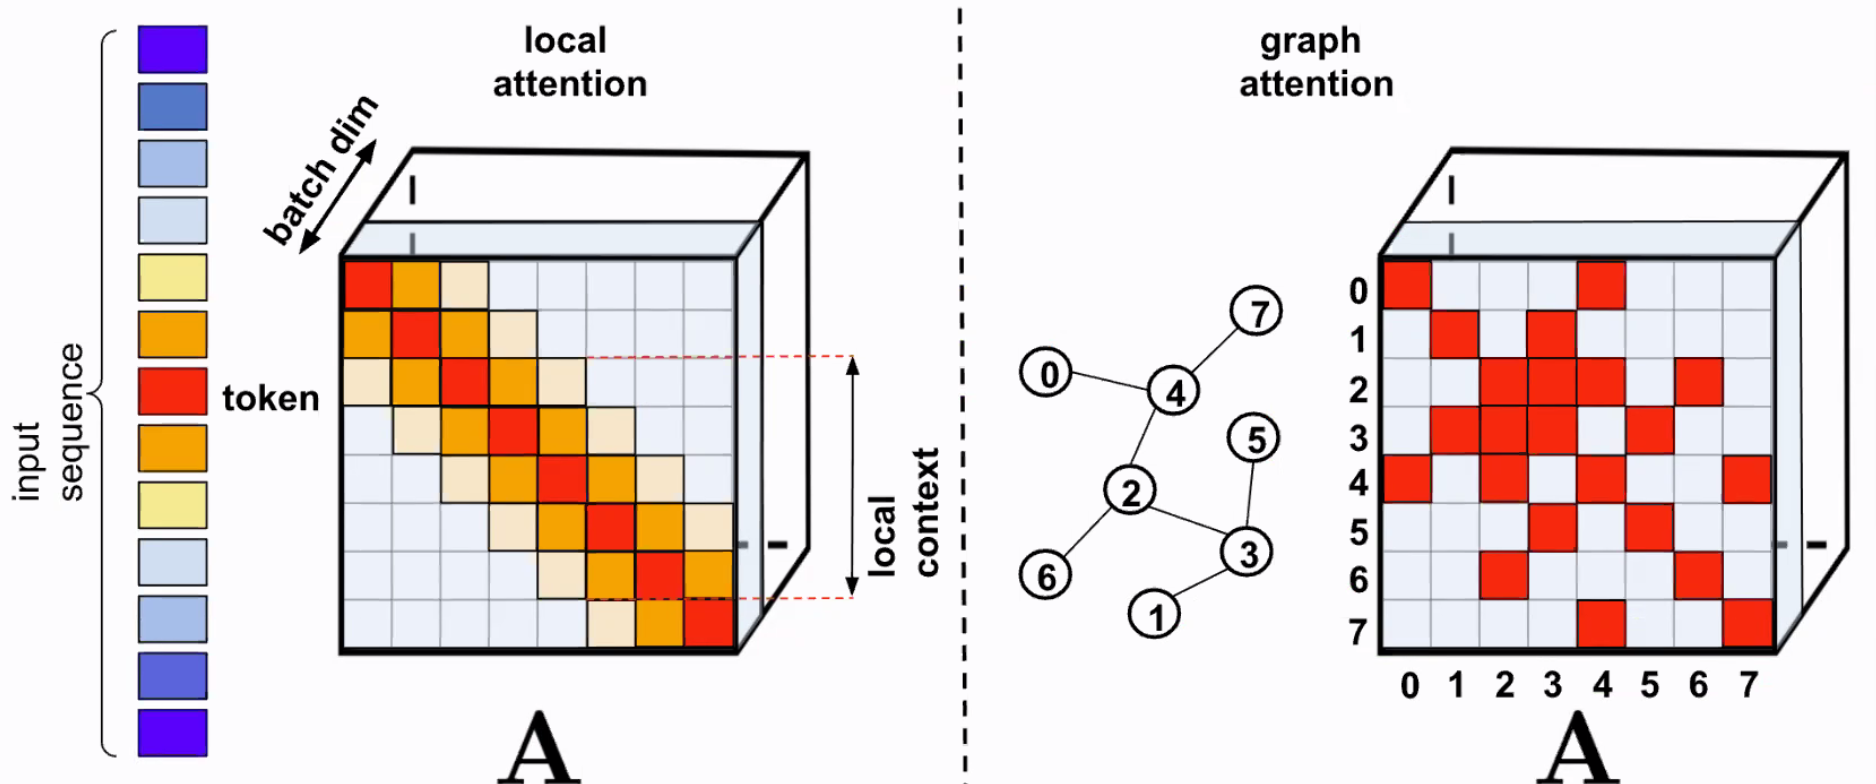
\includegraphics[width=0.9\textwidth]{local_attention.png}

One way to make the attention architecture more scalable would be to only look at local attention, or attention in the neighborhood of each token. Graph attention is another possibility. 	

We talked about how the  attention matrix could roughly be though of as a similarity matrix. In ML, we refer to similarity matrices as kernels. 


\subsubsection*{Terms to look up:}
\begin{itemize}
	\item dense attention vs. sparse attention
	\item attend (verb)
	\item attention matrix
	\item queries and keys in attention
	\item performer model
	\item kernelizable in ``attention is kernelizable''. Also, \href{https://en.wikipedia.org/wiki/Kernel_method}{kernel methods} in general
	\item partition function 
\end{itemize}


Usually, you take some row representation of you data.